\documentclass{beamer}
\usepackage[english,ngerman]{babel}
\usepackage[utf8]{inputenc}
\usepackage[T1]{fontenc}
\usepackage[autostyle,babel,german=guillemets,style=german]{csquotes}

%---------------------------------------------------------------------
% Globale Variabeln
%---------------------------------------------------------------------
\newcommand{\event}{Hochvolt Systeme}
\newcommand{\location}{Bochum}
\newcommand{\dt}{\today}
\newcommand{\x}[1]{\mathrm{#1}}  		
%---------------------------------------------------------------------

\usepackage[%
 backend=biber,%
 style=authoryear,%
 bibstyle=authoryear,%
 citestyle=authoryear,%
 natbib=false,%
 sorting=anyt,%
 sortcites=true,%
 hyperref=auto,%
 maxnames=3,%
 minnames=1,%
 refsection=subsection,%
 dashed=false%
]{biblatex}

\bibliography{bibo}
\setlength{\bibitemsep}{0.5em}

\defbibheading{bibliography}[\bibname]{%
\subsubsection*{#1}%
\markboth{#1}{#1}}

\usetheme[%
wiwi,
%nav,        		  	%% Schaltet die Navigationssymbole ein
%frutiger,				%% Ändert die Schrift in Frutiger
%mathpazo,				%% mathpazo Schrift
%mathptmx,				%% Times Schrift
colorful,    			%% Farbige Balken im infolines-Theme
%infoSub,				%% Aktiviert Infoline mit Subsections
infoline,				%% Aktiviert die Infoline über dem Frametitle
squares,     			%% Aufzaehlungspunkte rechteckig
nologo       			%% Kein Logo im Seitenhintergrund
]{FUH}

\title[Parameteridentifikation]{Ansätze zur Parameteridentifikation einer PMSM}

\author[Benjamin Ternes]%
{%
Benjamin Ternes
}

\institute{%
Hochschule Bochum\\
Fachbereich Elektrotechnik und Informatik}

\AtBeginSection[]{%
  \begin{frame}[plain] %<beamer>
    \frametitle{Agenda}
    \tableofcontents[currentsection]
     % \tableofcontents[sectionstyle=show/hide,subsectionstyle=hide/show/hide]
  \end{frame}
  % \addtocounter{framenumber}{-1}% If you don't want them to affect the slide number
}

\begin{document}

\begin{frame}[plain]
	\titlepage
\end{frame}

\begin{frame}[plain]{Autor}
Benjamin Ternes
\begin{itemize}
	\item VDE (Verband der Elektrotechnik Elektronik Informationstechnik e.\ V.\ ) Mitglied, Bezirk Düsseldorf	\url{http://www.vde.com/}
	\item IEEE \url{https://www.ieee.org/index.html}
	\item Dante e.\ V.\ Mitglied~--~Deutschsprachige Anwendervereinigung TeX e.\ V.\ \url{http://www.date.de/}
\end{itemize}
\vspace{1cm}
Publikationen:\\
\fullcite{ternes2012}
\end{frame}

\begin{frame}[plain]{Agenda}
	\tableofcontents
\end{frame}

\section{Einleitung}
\begin{frame}{Allgemeines}
\begin{itemize}
\pause \item PMSM in einer Vielzahl unterschiedlicher Anwendungen (vorallem kleinen bis mittleren Leistungen)
\pause \item Hochdynamische Antriebsmotoren (hochdynamische Regelung)
\pause \item Hochdynamische Regelungen benötigen die »Induktivitäten« der Maschine (abh. vom momentanen Strom)
\pause \item Flussverkettung $\Psi$ ändert sich aufgrund von Alterungserscheinungen und Temperaturveränderungen
\pause \item Ohmscher Ständerwiderstand kann sich im Betrieb fast verdoppeln
\end{itemize}
\end{frame}

\section{Mathematisches Modell einer PMSM}
\begin{frame}[plain]{Koordinatensysteme}
\begin{figure}[!t]
\centering
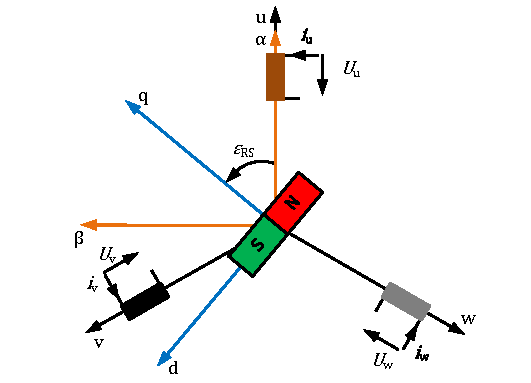
\includegraphics[width=\textwidth]{img/synchron-grundlage}
\caption{Graphische Veranschaulichung der verschiedenen Koordinatensysteme, ständerfest $(\alpha, \beta)$ und rotorfest $(d, q)$.}
\label{fig:synchron-grundlage}
\end{figure}
\end{frame}

\subsection{Linearisierte Gleichungen}
\begin{frame}{Linearisierte Gleichungen}
\begin{itemize}
\pause \item Definitionsgemäß sind keine Sättigungserscheinungen vorhanden \autocites{mullerII2008}{schroder2001}
\pause \item Alle elektrischen Parameter einer PMSM und damit auch die Induktivitäten sind konstant
\end{itemize}

\pause{\begin{align}
\Psi_\x{d} &= \Psi_\x{pm} + L_\x{d} i_\x{d} \label{eqn:psid}\\
\Psi_\x{q} &= L_\x{q} i_\x{q} \label{eqn:psiq} \\
M_\x{i} &= \frac{3p}{2}(\Psi_\x{d} i_\x{q} - \Psi_\x{q} i_\x{d}) \label{drehmoment}
\end{align}

(vgl.~\textcite{schroder2001})}
\end{frame}

\begin{frame}{Linearisierte Gleichungen}\label{fol:lin-gleichungen}
\begin{block}{Spannungsgleichungen des linearisierten Modells}
\begin{align}
u_\x{d} &= R_\x{1} i_\x{d} + L_\x{d} \frac{\x{d}i_\x{d}}{\x{d}t} - \omega_\x{el}L_\x{q} i_\x{q}  \label{uq-allg} \\ 
u_\x{q} &= R_\x{1} i_\x{q} + L_\x{q} \frac{\x{d}i_\x{q}}{\x{d}t} + \omega_\x{el}L_\x{d} i_\x{d} + \omega_\x{el}\Psi_\x{pm} \label{ud-allg} \\ 
M_\x{i} &= \frac{3p}{2}(\Psi_\x{pm} i_\x{q} + (L_\x{d} - L_\x{q})i_\x{d} i_\x{q})
\end{align}
(vgl.~\textcite{schroder2001})
\end{block}
\end{frame}

\begin{frame}[plain]{Linearisierte Gleichungen}
\begin{figure}[!t]
\centering
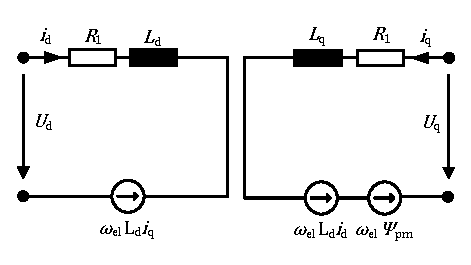
\includegraphics[width=\textwidth]{img/spannungsgleichungen}
\caption{Graphische Darstellung der Gleichungen Gl.~(\ref{uq-allg}) und Gl.~(\ref{ud-allg}).}
\label{fig:synchron-grundlage}
\end{figure}
\end{frame}

\subsection{Allgemeine Gleichungen}
\begin{frame}{Allgemeine Gleichungen}
\begin{itemize}
\pause \item Induktivitäten ändern sich $\rightarrow$ abhängigkeit: Belastung
\pause \item Grund: Sättigungseffekte, Kreuzkopplung~--~entsteht durch Beeinflussung der verkoppelten Induktivitäten
\pause \item z.\ B.\ in der realen Maschine verlaufen die Ströme $i_\x{d}$ und $i_\x{q}$ in dem gleichen Ständerblech \autocite{Kellner2012}
\pause \item Bei Verwendung der linearen Gleichungen (s.~h.~Folie~\ref{fol:lin-gleichungen}) werden Sättigungseffekte vernachlässigt
\pause \item Unter Berücksichtigung der Eisenverluste bzw. Wirbelstromverluste reichen die Gleichungen nicht mehr aus
\end{itemize}
\end{frame}

\begin{frame}{Neue Gleichungen für $\Psi_\x{d}$ und $\Psi_\x{q}$}\label{fol:allg-flussverkettung}
\begin{itemize}
\pause \item Einige Ansätze unterteilen die Induktivitäten in Selbst- und Gegeninduktivitäten \autocite{stumberger_evaluation_2003}
\pause \item Dabei sind sowohl die Selbst- als auch die Gegeninduktivität jeweils von den Strömen abhängig $\rightarrow$ Hysterese
\end{itemize}

\pause{\begin{align}
\Psi_\x{d} &= \Psi_\x{pm} + L_\x{dd}^{\xi}(i_\x{d})\cdot i_\x{d} + L_\x{dq}^{\xi}(i_\x{d} ,i_\x{q})\cdot i_\x{q} \\
\Psi_\x{q} &= L_\x{qq}^{\xi}(i_\x{q})\cdot i_\x{q} + L_\x{qd}^{\xi}(i_\x{d} ,i_\x{q})\cdot i_\x{d}
\end{align}

(vgl.~\textcite{stumberger_evaluation_2003})}

\end{frame}

\begin{frame}{Darstellungsweise der Induktivitäten}\label{fol:darstellung-induktiv}
\pause Nach \textcite{Kellner2012} ist es möglich die Induktivitäten intuitiv darzustellen als:

\pause{\begin{align}
L_\x{d}^{(i_\x{d},i_\x{q})} &= L_\x{dd}^{\xi}(i_\x{d}) + L_\x{dq}^{\xi}(i_\x{d},i_\x{q})\cdot\frac{i_\x{q}}{i_\x{d}} \\
L_\x{q}^{(i_\x{d},i_\x{q})} &= L_\x{qq}^{\xi}(i_\x{q}) + L_\x{qd}^{\xi}(i_\x{d},i_\x{q})\cdot\frac{i_\x{d}}{i_\x{q}}
\end{align}}

\end{frame}

\begin{frame}
\pause Anhand Folie~\ref{fol:darstellung-induktiv} lassen sich damit die Flussverkettung von Folie~\ref{fol:allg-flussverkettung} vereinfachen:
\vspace*{0.5cm}
\pause{\begin{block}{Flussverkettungen der allgemeinen Maschinengleichungen}
\begin{align}
\Psi_\x{d}^{(i_\x{d},i_\x{q})} &= \Psi_\x{pm}^{(i_\x{d},i_\x{q})} + L_\x{d}^{(i_\x{d},i_\x{q})}\cdot i_\x{d} \\
\Psi_\x{q}^{(i_\x{d},i_\x{q})} &= L_\x{q}^{(i_\x{d},i_\x{q})}\cdot i_\x{q}
\end{align}
Diese Darstellungsweise ist kürzer und übersichtlicher
\end{block}}

\pause $\rightarrow$ Mehrwert wegen Trennung der Selbst- und Gegeninduktivität? \autocite{Kellner2012}.
\end{frame}

\begin{frame}{Allgemeine Maschinengleichungen in Zustandsform}
Insgesamt sieht das Gleichungssystem zum identifizieren der Parameter einer PMSM wie folgt aus:

\begin{align}
\left( \begin{array}{c} u_\x{d} \\ u_\x{q} \end{array} \right) &= \left( \begin{array}{cc} R_\x{1} & -\omega_\x{el}L_\x{q}^{(i_\x{d},i_\x{q})} \\ \omega_\x{el}L_\x{d}^{(i_\x{d},i_\x{q})} & R_\x{1} \end{array} \right) \left(\begin{array}{c} i_\x{d} \\ i_\x{q} \end{array}\right) \label{eqn:allg-spannungsgleichung} \\ 
 &\ldots + \underbrace{\left( \begin{array}{cc} L_\x{dd}^{(i_\x{d},i_\x{q})} & L_\x{dq}^{(i_\x{d},i_\x{q})} \\ L_\x{qd}^{(i_\x{d},i_\x{q})} & L_\x{qq}^{(i_\x{d},i_\x{q})} \end{array}\right)}_{\text{differentielle Induktivitäten}} \left(\begin{array}{c} i_\x{d} \\ i_\x{q} \end{array} \right) \nonumber \\ 
& \ldots + \left( \begin{array}{c} \frac{\x{\partial}}{\x{\partial }t} \Psi_\x{pm}^{(i_\x{q})} \\ \omega_\x{el} \Psi_\x{pm}^{(i_\x{q})} \nonumber \end{array}  \right) \nonumber
\end{align}
\end{frame}

\begin{frame}[plain]{Spannungsgleichungen der allgemeinen Maschinengleichungen}
\begin{figure}[!h]
\centering
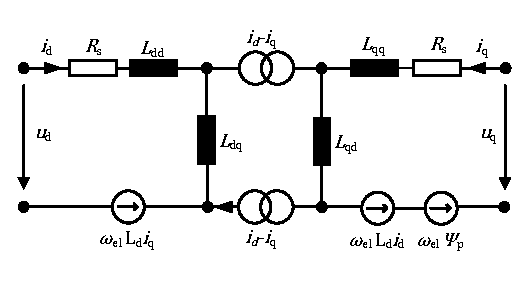
\includegraphics[width=\textwidth]{img/allg-spannungsgleichung}
\caption{Graphische Darstellung der Gleichungen (Gl.~\ref{eqn:allg-spannungsgleichung}).}
\label{fig:allg-spannungsgleichung}
\end{figure}
\end{frame}

\section{Ansätze zur Identifikation}
\begin{frame}{Vorwissen}
\begin{itemize}
\pause \item Warum?
\vspace*{2cm}
\pause \item Was ist notwendig?
\end{itemize}
\end{frame}

\subsection{Bestimmung der Rotorlage}
\begin{frame}{Geberlose Regelung? Inkrementalgeber? Resolver? $\rightarrow$ ???}
	\begin{itemize}
		\pause \item Vorteil einer geberlosen Regelung: Keinen Wartungsaufwand, geringere Kosten $\rightarrow$ keine Rotorposition bei niedrigen Drehzahlen?
		\pause \item Vorteil eines Resolvers: Absolutwert der Rotorposition $\rightarrow$ Wartungsaufwand und höhere Kosten
		\pause \item Ein Inkrementalgeber ist nicht sinnvoll, zu ungenau.
	\end{itemize}
\end{frame}

\subsection{Ansätze zur Identifikation der Induktivitäten, Ständerwiderstand und Flussverkettung}\label{fol:ansatz-induktiv}
\begin{frame}{Ansätze zur Identifikation}
	\begin{itemize}
		\item Unterteilung der Induktivitäten in: absolute und differentielle Induktivitäten
		\item Offline? Online?
	\end{itemize}

\pause{
\begin{quote}
	\enquote{Zum einen ändern sich die Induktivitäten im Wesentlichen nur abhängig von den Strömen $i_\x{d}$ und $i_\x{q}$, kaum aufgrund von anderen äußeren Umgebungseinflüssen beziehungsweise Prüfstandsparametern, wie zum Beispiel Temperatur oder Drehzahl des Systems \autocite[S.~79]{Kellner2012}.}
\end{quote}
	}
	
\end{frame}

%\subsection{Ansätze zur Identifikation des Ständerwiderstand}
\begin{frame}{Onlinemessverfahren}

Aus den Erkenntnissen von Folie~\ref{fol:ansatz-induktiv} ist eine Onlinemessung nicht erforderlich~--~im Gegensatz zur Ständeridentifikation

\begin{itemize}
	\item Onlineverfahren sind entweder gar keine richtigen \enquote{online}-Verfahren oder haben zweifelhafte Stabilität und Genauigkeit \autocite{underwood_online_2010}
\end{itemize}
\end{frame}

\begin{frame}
\begin{alertblock}{Wichtig}
	Induktivitäten können offline gemessen werden, der Ständerwiderstand kann nur online bestimmt werden:
\end{alertblock}

	\begin{quote}
		\enquote{Using an online parameter estimation algorithm allows the controller to have precise parameter estimates even when these are subject to perturbation, regardless of its origin. Consequently, phenomena like temperature effects and cross-saturation can be accounted for through their effect on the machine parameters, which is difficult with an offline method \autocite[S.~1]{underwood_online_2010}.}
	\end{quote}

\end{frame}

\section{Parameterfehler}
\begin{frame}

\end{frame}

\begin{frame}{Block}
\begin{block}{Title}
Das ist ein Block mit Aufzählungen:
\begin{itemize}
	\item 1
	\item 2
	\item 3
	\item \ldots
\end{itemize}
\end{block}
\end{frame}

\section*{Bibliography}
\begin{frame}[allowframebreaks]{Bibliography}
%\nocite{*}
\printbibliography
\end{frame}

\end{document}